%%%%%%%%%%%%%%%%%%%%%%%%%%%%%%%%%%%%%%%%%%%%%%%%%%%%%%%%%%%%
%%% ELIFE ARTICLE TEMPLATE
%%%%%%%%%%%%%%%%%%%%%%%%%%%%%%%%%%%%%%%%%%%%%%%%%%%%%%%%%%%%
%%% PREAMBLE
\documentclass[9pt,lineno]{elife}
% Use the onehalfspacing option for 1.5 line spacing
% Use the doublespacing option for 2.0 line spacing
% Please note that these options may affect formatting.
% Additionally, the use of the \newcommand function should be limited.

\usepackage{minted}
\usepackage{tcolorbox}
\usepackage{etoolbox}
% \BeforeBeginEnvironment{minted}{\begin{tcolorbox}}
% \AfterEndEnvironment{minted}{\end{tcolorbox}}

% Systematise how we typeset elements of the API (functions, variables, etc)
\newcommand{\sgapi}[1]{\texttt{#1}}
\newcommand{\toolname}[1]{\texttt{#1}}

\newcommand{\sgkit}{\texttt{sgkit}}

%%%%%%%%%%%%%%%%%%%%%%%%%%%%%%%%%%%%%%%%%%%%%%%%%%%%%%%%%%%%
%%% ARTICLE SETUP
%%%%%%%%%%%%%%%%%%%%%%%%%%%%%%%%%%%%%%%%%%%%%%%%%%%%%%%%%%%%
\title{Scalable statistical genetic data analysis in Python}

\author[1]{Eric Czech}
\author[1,2\authfn{1}\authfn{3}]{Firstname Middlename Familyname}
\author[2\authfn{1}\authfn{4}]{Firstname Initials Surname}
\author[2*]{Firstname Surname}
\affil[1]{Related Sciences LLC}
\affil[2]{Institution 2}

\corr{email1@example.com}{FMS}
\corr{email2@example.com}{FS}

\contrib[\authfn{1}]{These authors contributed equally to this work}
\contrib[\authfn{2}]{These authors also contributed equally to this work}

\presentadd[\authfn{3}]{Department, Institute, Country}
\presentadd[\authfn{4}]{Department, Institute, Country}
% \presentadd[\authfn{5}]{eLife Sciences editorial Office, eLife Sciences, Cambridge, United Kingdom}

%%%%%%%%%%%%%%%%%%%%%%%%%%%%%%%%%%%%%%%%%%%%%%%%%%%%%%%%%%%%
%%% ARTICLE START
%%%%%%%%%%%%%%%%%%%%%%%%%%%%%%%%%%%%%%%%%%%%%%%%%%%%%%%%%%%%

\begin{document}

\maketitle

% Please provide an abstract of no more than 150 words. Your abstract should
% explain the main contributions of your article, and should not contain any
% material that is not included in the main text.

\begin{abstract}
The PyData ecosystem is an umbrella term covering Python packages based on a
broad range of modern techniques, such as chunk-compressed columnar data
storage, just-in-time compilation of numerical code, and scaling of
calculations across clusters of computers. Together, these technologies have
been successfully applied in scientific applications using data at the petabyte
scale. These technologies, and the many benefits that they provide, however,
have not been successfully applied in the field of genomics, which is currently
making the transition to working at petabyte scale. We present sgkit, a Python
package designed to bring the benefits of the PyData ecosystem to genomics,
allowing users to efficiently analyse large-scale data using familiar tools. We
discuss the underlying design principles of these technologies and illustrate
their suitability in genetics and genomics applications, via examples on
large-scale datasets such as UK Biobank.
\end{abstract}

\section{Introduction}

% This current phrasing would annoy people, just spewing this
% out to roughly say what I think is relevant, we can refine later.
The study of genetics is currently transforming into a true big-data science.
Since the Human Genome Project, genomics has required working with
signicant volumes of data and the specialised methods
required to transform the raw biological signals into analysable data,
such as assembly[cite], mapping[cite] and variant calling[cite] are compute intensive.
However, beyond these initial steps required to generate the data, the actual
analysis of the genetic variation could typically be performed on a single
computer, and often with ad-hoc software written using shell utilities
and scripting languages such as Perl.
From the Human Genome Project, through 1000 Genomes, and now with
population scale genomics datasets such as UK Biobank, GeL, etc,
the requirements for analysing the data have far outgrown these
methods. Simple queries can require minutes to complete, which
has a negative effect on researcher productivity, as well as limiting
the analyses that can be performed. The financial cost of working
with such datasets is also substantial, which limits accessibility
to an elite set of well-funded groups.

[Summary of what we do and paper roadmap]

In this paper we present sgkit, a Python library for large-scale genetic data
analysis that supports efficient and convenient distributed computation based
on open data formats and established technologies. We begin by examining the
fundamental question of how we can store observed genotypes for millions of
samples and hundreds of millions of variant sites in a way that is compact,
supports efficient retrieval for subsets of both samples and sites, and leads
to efficient distributed computation. We demonstrate that the straightforward
approach of storing genotypes in compressed rectangular chunks using the Zarr
library enables efficient access by sample, and yields compression levels and
computation speeds similar to specialised methods for genetic data. These
chunks also provide
a natural unit % FIXME "unit" is the wrong word
to parallelise work over, and by using the Dask library sgkit can easily and
transparently execute tasks concurrently within a single computer or across a
large cluster. Concurrent and distributed programming is notoriously difficult,
but Dask's high-level array-oriented operations, coupled with just-in-time
(JIT) compilation via numba~\citep{lam2015numba}, makes it straightforward to
write performant distributed code in Python.
Storing and processing genotype data is of course only one part of
genetic data analysis, and real-world analyses require large volumes
of additional data associated with variants, samples and genotypes calls.
To help manage this complexity
the basic unit of sgkit's interface is an Xarray
dataset~\citep{hoyer2017xarray}, which provides a flexible container
for labelled multi-dimensional arrays. Thus, arbitrary numerical data
can be associated with any of the relevant dimensions, and stored
efficiently in chunked Zarr format.

Using these fundamental building blocks sgkit currently provides
functionality across four key themes of general quality-control,
statistical, population and quantitative genetics. In
each case we briefly discuss available software, and showcase
the functionality via case-studies.
% Note: wishlist, just writing down some stuff that sounds good!
% Also four-key themes doesn't quite fit with 5 sections mentioned
% below - it's a WIP.
We first demonstrate interactive quality-control of [large dataset]
on [cluster], demonstrating how users can quickly summarise
large-scale data in a Jupyter notebook. We then illustrate the
statistical genetics functionality by performing a GWAS
on [something]. We showcase support for
population genetic data by [doing something from one of Alistairs
notebooks?].
We then demonstrate support for quantitative genetics
applications by applying relatedness matrix functions to [something].
% Note: it would be quite neat if we could say this is support
% for phylogenetics operations. Coupled with upstream SeqData
% we might actually be able to do this for some public SARS-CoV-2
% data or something, and make a neighbour joining tree using
% scipy (which is a terrible method, so would have to fully
% acknowledge).
Finally, demonstrate sgkit's support for heterogenous computing
and the general potential for using GPUs by computing a
pairwise distance matrix for [something], and demonstrate
X-fold speedup using our GPU implementation.

% Maybe this belongs in the discussion - we can leave it here for now.
Sgkit builds on the four key technologies of Zarr, Dask, Numba and Xarray,
widely used throughout the sciences, to bring efficient large-scale
genetics computation within the reach of many.
Sgkit is by design an open ecosystem.
The data model is well-documented,
based on open standards, and extensible to include arbitrary additional
variables and dimensions. Users are not restricted to a limited palate
of analyses, but have the full power of the Python data-science stack
available, and can write their own operations in terms of distributed
array operations or optimised numerical code. Finally, sgkit's
development model is open, with a codebase that is specifically
designed for ease of contribution,
% This is horrible, put in something better later.
and development processes informed
by combined decades of experience in open-source projects.


\section{Results}
Here is a quick rundown of the sections and what they do:

\paragraph{Storing genetic variation data}
High level discussion of
strategies used to store genotype matrix and accompanying metadata.
Emphasis on access by variant, not sample. Introduce Zarr, and
refer to Fig~\ref{fig-data-storage}A to explain columnar storage,
and Fig~\ref{fig-data-storage}B to show that is competitive
with highly specialised approaches.
Note that the FC simulated dataset is probably a best-case
scenario for methods specialised to patterns in the genotype matrix.
Discuss storing additional data, and advantages of the
columnar approach (refs to genomics tools that do the same).

\paragraph{Computing on the genotype matrix}
Compressing data isn't ultimately the point - we want to use it.
We discuss the problem of running computations on the entire
genotype matrix, and how different formats limit what can be done.
We illustrate the discussion by the afdist operation from
the bcftools plugins package. This is perhaps a contrived example, but
we chose it because it requires examining the entire genotype matrix
and there is an efficient implementation available in bcftools.
It is also a good example because the standard approach of
divvying up the genome into chunks via HPC schedulers or workflow
managers is quite tricky.
We discuss the software development aspect, and how we developed
the afdist-savvy program. We discuss the inherent limitations
of the decode-to-vcf strategy, and how this inevitably
leads to bottlenecks. We discuss parallelism, and why
bcftools and genozip can make limited use of available cores.
Also that single-machine parallelism is inevitably constrained
by IO (which is why savvy's thread utilisation drops off).
Figure: \ref{fig-whole-matrix-compute}. Also
supplementary figure ~\ref{fig-whole-matrix-compute-supplemental}.

\paragraph{Subsetting the genotype matrix}
Existing work overwhelmingly emphasises accessibility by variant.
We demonstrate that sgkit/zarr is good for getting subsets
in terms of both variants and samples via afdist on various subsets.
Discuss why storing AF values for crude population groupings is
intrinsically bad, and that it should be easy to do calculations
on aribitrary subsets. Also participants regularly drop-out of
large studies like UKB - do you update the AF values each time?

\paragraph{Distributed computation}
Why do we need distributed compute? Summary of current
approaches (chunk up along the genome using HPC or workflow
managers). Advantages of true distributed compute, MapReduce
etc. Summary of earlier efforts like ADAM.
Discuss Hail. It's awesome, has enabled current
generation of mega-scale projects. Drawbacks are the
architecture has emphasised performance etc over adaptability
and simplicity. File format is undocumented, etc.
Discuss why the sgkit architecture is suited to distributed
computation. Discuss Zarr's use in cloud stores, and existing
deployments. Discuss Dask.
We do not attempt a head-to-head performance comparison with
Hail here, but defer to Liangde's thesis~\citep{li2022efficient}
with brief summary.
Forward ref to following sections on applications to demonstate
sgkit in a distributed context.

\paragraph{Quality control of large datasets}
Outline the importance of QC, and existing approaches.
Summarise sgkit's general QC capabilities.
We demonstrate sgkit on quality control operations on a large
real dataset. We convert large messy VCF with lots of additional
fields. Quote file size numbers. We do some QC operations on
the dataset, using a good size distributed cluster, using
some of the additional fields. Quote times. Discuss Xarray
here, and possibly illustrate the labelled dimensioned arrays
here via a figure (perhaps a screenshot/pdf conversion of
a Jupyter notebook rendering of the big messy dataset,
showing the various fields).

\paragraph{Statistical genetics}
Quick summary of statgen and existing toolchain.
Summarise sgkit's statgen capabilities.
Demonstrate sgkit doing a GWAS on real data using distributed cluster.
Quote numbers.

\paragraph{Population genetics}
Quick summary of popgen and existing toolchain.
Summarise sgkit's popgen capabilities.
Demonstrate
sgkit doing popgen analysis based on MalariaGEN data (on cluster?)
Quote numbers.

\paragraph{Quantitative genetics}
Quick summary of quantgen and existing toolchain.
Summarise sgkit's quantgen capabilities. Emphasise the importance
of mixed ploidy support.
Demonstrate sgkit doing some relatedness matrix analyses.
Quote numbers, possibly relative to existing tools.

\paragraph{Phylogenetics}
Quick summary of phylogenetics and existing toolchain.
Phylo is not one of sgkit's core capabilities, but there's no
reason it can't support important. Workflows are also becoming
VCF-based, and massive datasets like SC2 would definitely
benefit from the ability to distribute.

We demonstrate the potential by doing computing pairwise
distance matrix from XX samples, and creating a neighbour
joining tree using scipy (which we emphasise is a terrible
idea, but still). We showcase sgkit's support for heterogenous
computing by getting an X-fold speedup on a GPU.

\section{Older text}

\subsection{Chunked storage and distributed computation}
How we store genetic data fundamentally affects how computation
can be structured, and ultimately the scalability of the calculations
we wish to perform. Classically, genetic variation data is stored via one
of two strategies. The first strategy, epitomised by
VCF~\citep{danecek2011variant} encodes all the data for a given
variant in a record, and then stores these records consecutively on file
(optionally compressed). This record-oriented approach maps well to the
powerful Unix pipelines abstraction and
has proven to be very successful.
The second classical strategy, epitomised
by the \texttt{plink} BED format~\citep{purcell2007plink}, is to
store genotype data in a structured binary format that can be
accessed directly. This memory-map approach tends to
be much faster to access, but leads to larger files and is more
limited in what can be represented. There are advantages and
disadvantages to both approaches, but one problem fundamentally
limits their utility for modern datasets: neither is well suited to
scaling-out across multiple machines.

[Probably need a paragraph here on what we've done classically
by splitting by variant. This was the dominant dimension, so that
worked fine. Now we need to also think about access-by-sample]

Given the scale of modern datasets, the ability to perform
calculations in parallel on multiple CPU cores
is now a basic prerequisite, and
running concurrently on multiple computers in a cluster
is increasingly becoming necessary. [For interactive analysis? People have
been doing concurrent computing with HPC clusters forever.]
Record-oriented variant storage such as VCF is not suitable
for  distributed computing because although it is relatively
straightforward to break workloads up by variant, we cannot efficiently
split by sample (see the section on Columnar Data below for details).
Storing data in a memory-mapped manner, where the genotypes
for each variant are written consecutive consecutively to a file,
suffers from the same problem. Although it is useful to conceptualise
the genotype matrix as two-dimensional, it is important to remember
that computer memory and file storage is ultimately one-dimensonal.
For example, plink's memory-mapped data layout linearises the 2D
genotype matrix by writing [TODO check] $n$ bytes representing
the genotypes for all samples at a variant position consecutively.
Because the genotypes for a given variant index can be found
in contiguous blocks at easily computable offsets from
this initial location in memory,
accessing the genotypes for a given variant is very efficient.
However, accessing the genotypes for a given sample at every
variant position is much less efficient because each of the $m$ bytes we
must read are $n$ bytes apart in the file.
In the distributed context, this often means
that each compute node  in a
cluster must effectively read the entire file in order to obtain the
data for a subset of samples. In practise, this means that calculations
are limited by I/0 bandwidth.

\begin{figure}
\begin{tabular}{cc}
% The source for this figure is a google drawing
% Currently using
% https://docs.google.com/drawings/d/1NheB6LCvvkB4C0nAoSFwoYVZ3mtOPaseGmg_mZvcQ8I
% See https://github.com/pystatgen/sgkit-publication/issues/21 for
% discussion
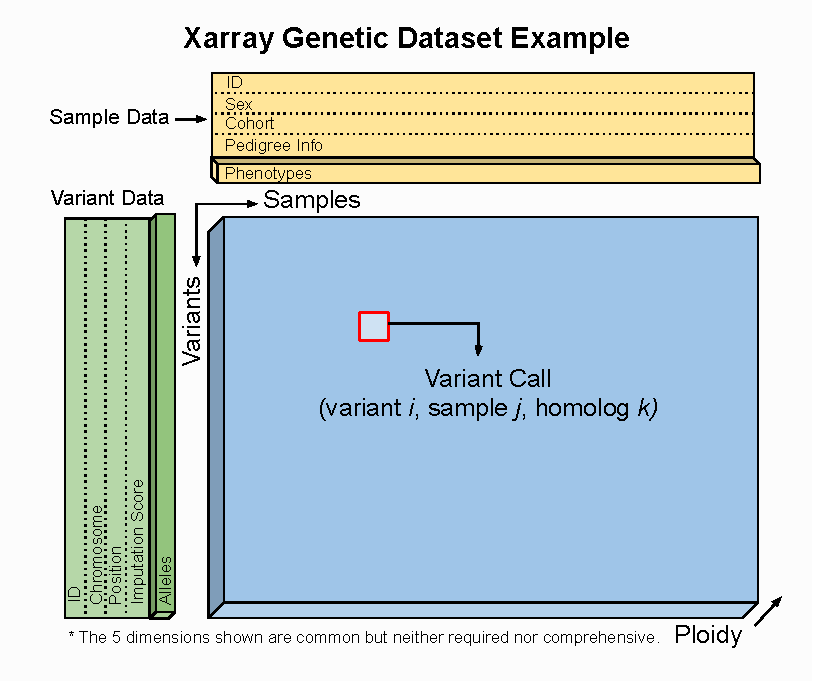
\includegraphics[width=6cm]{diagrams/sgkit_xarray_diagram.pdf} &
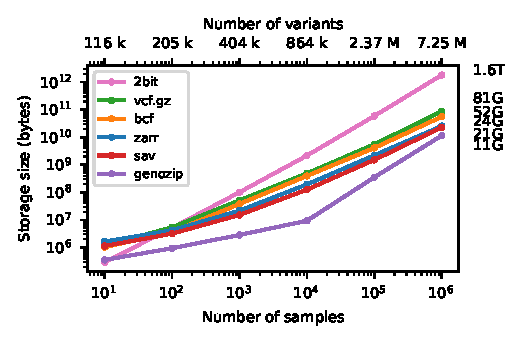
\includegraphics[width=6cm]{figures/data-scaling}
\end{tabular}
\caption{Chunked compressed storage of the genotype matrix using Zarr.
(A) Schematic of the chunked array storage used in sgkit
[Note: wrong fig. See
\url{https://github.com/pystatgen/sgkit-publication/issues/46} for
proposed update].
(B) Compression performance compared with BCF, savvy and genozip
based on simulated data (see text for details).
\label{fig-data-storage}}
\end{figure}

A simple and elegant solution to providing efficient access to such
large matrices across multiple dimensions is to store rectangular
\emph{chunks} rather than entire rows or columns. This is illustrated
in Fig~\ref{fig-data-storage}, where we show the basic approach
used by sgkit. By storing data in these regular chunks, we
can efficiently access data for both specific variants \emph{and}
samples.

Additionally, we can compress the individual chunks [more details].

This general strategy for storing multidimensional numerical data
has been in use for many years~\citep{folk2011overview}

This maps well to distributed computing because Zarr provides a
very flexible approach to storing the chunks. By using a native cloud store
for these chunks, compute nodes can directly access the chunks that
are needed, and not read irrelevant data.
[TODO flesh out and more stuff.]


\subsection{Scaling up interactive analysis}
The storage and analysis of datasets consisting of hundreds of
thousands of genomes presents major challenges.
Fig.~\ref{fig-data-storage} shows the performance of \toolname{sgkit}
in terms of storage space and computation time  on a simple benchmark (see
below for details) with increasing
numbers of samples, contrasting with the standard BCF file format
and \toolname{bcftools} utility.
The dataset used is a subset of the
ultra-realistic simulations of 1.4 million French-Canadians
provided by~\citet{anderson2023genes}, which is freely avilable
and has been shown to
accurately reflect fine-scaled demographic structure.
Although
simulations can never capture the full richness of real data,
this resource certainly reflects the patterns of allele frequency
and correlation structure that we would expect in large-scale
human studies, and provides a useful and reproducable benchmark.
Note that as we increase the sample size, the number of variant
sites also increases [following basic popgen principles?].

The scale of present-day genomic data means that compact
storage is of paramount importance, and reductions in storage space
can make a significant difference in overall costs.
Fig.~\ref{fig-data-storage}A shows that the
compressed-chunked-array Zarr format used by \toolname{sgkit} results
in significantly smaller file-sizes than BCF (encoded using
\texttt{bcftools view -O b}; we used \toolname{bcftools}
version 1.18 throughout). At the extreme, when we have 1M
samples, we require XGB for the BCF file and a total of YGB
for the \toolname{sgkit} version. Note that under the default
directory based Zarr store this results in XX files of around
y KB each to store the chunks. Different Zarr storage engines
can be used, varying from a ZipFile which keeps the entire
dataset in a single file to a cloud store [details] which stores
chunks in [a cloud store]. The chunk size is a parameter and
can be tuned. [bit more detail here].

\begin{figure}
\begin{tabular}{cc}
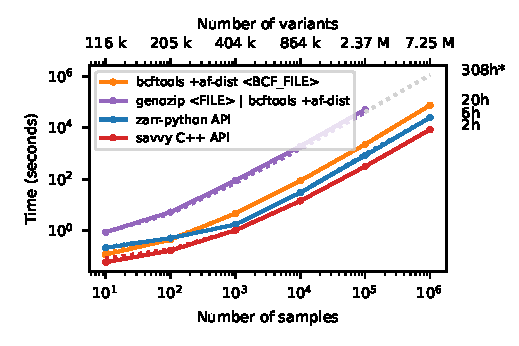
\includegraphics[width=6cm]{figures/whole-matrix-compute} &
\begin{tcolorbox}[width=7cm]
\begin{minted}[fontsize=\footnotesize]{python}
def sgkit_afdist(ds, num_bins=10):
    ds_vs = sgkit.variant_stats(ds).compute()
    bins = np.linspace(0, 1.0, num_bins + 1)
    bins[-1] += 0.01
    af = ds_vs.variant_allele_frequency.values[:, 1]
    pRA = 2 * af * (1 - af)
    pAA = af * af
    hets = ds_vs.variant_n_het.values
    homs = ds_vs.variant_n_hom_alt.values
    a = np.bincount(
        np.digitize(pRA, bins),
        weights=hets,
        minlength=num_bins + 1)
    b = np.bincount(
        np.digitize(pAA, bins),
        weights=homs,
        minlength=num_bins + 1)
    count = (a + b).astype(int)
    return pd.DataFrame({
        "start": bins[:-1],
        "stop": bins[1:],
        "prob_dist":
        count[1:]})

ds = sgkit.load_dataset(ds_path)
df = sgkit_afdist(ds)
\end{minted}
\end{tcolorbox}
\end{tabular}
\caption{Whole-matrix compute performance with increasing sample size.
(A) Total CPU time required to run \texttt{bcftools +afdist}
and equivalent operations in a single thread for various tools.
Elapsed time is also reported (dotted line).
(B) Relative speedup with 8 threads.
(C) The source code used for the sgkit version of afdist used in these
benchmarks. See Figure~\ref{fig-whole-matrix-compute-supplemental} for
more detailed comparisons with different numbers of threads, and comparing
the effects of HDD vs SSD storage.
\label{fig-whole-matrix-compute}}
\end{figure}

The scale of modern genomic datasets also means that calculations must
be parallelised. This is illustrated in Fig.~\ref{fig-whole-matrix-compute}B,
where we compare the performance of a simple calculation requiring
the examination of all genotypes using \toolname{bcftools}
and \texttt{sgkit}. Interactive analysis is only possible through
parallelisation, as optimised single-threaded code
is simply not fast enough.
Although it is relatively straightforward to split calculations across
the genome using tools like \toolname{bcftools}, the process
is quite manual, and often involves working with HPC schedulers
or workflow managers [this is very rough, just seeing where it goes].
Splitting the workload \emph{by sample} however, is much more
difficult. Parallelisation by variant and sample is an inherent
part of \texttt{sgkit}'s design---the variant matrix is chunked
in two dimensions, and Dask transparently maps computations to these
chunks.
Fig.~\ref{fig-whole-matrix-compute}B shows how \texttt{sgkit} scales
on a single server, and how computation time decreases as we use
more threads. In contrast, using threads with
\toolname{bcftools} (via the XXX option) makes almost no difference
because computational model is inherently sequential, and additional threads
are only used to facilitate decompression.
As we see in section XXX,
a major advantage of \texttt{sgkit} is that it not only supports
scaling \emph{up} within a server, but also scaling \emph{out}
across multiple servers.

The ability to
run pre-defined analyses interactively on very large datasets by
transparently distributing across a cluster is a major boost to
researcher productivity. The ability to define one's \emph{own}
analyses using familiar Python data-science tools and libraries,
and to similarly distribute across a cluster (with single-threaded
speed close to native compiled code) is a game-changer [say better].
Fig.~\ref{fig-whole-matrix-compute}C shows the code used in the benchmark
for \toolname{sgkit} in Fig.~\ref{fig-whole-matrix-compute}B. The heavy
computation here is done in the \texttt{variant\_stats(ds)} function,
which computes a set of variables summarising each of the variants
by examining the entire variant matrix.
These variables are mostly one-dimensional, and can thefore
be processed `in-core' using numpy methods very effectively.
For example, we \texttt{variant\_n\_het} the number of heterozygous samples
in Fig.~\ref{fig-whole-matrix-compute}C. For $n=10^6$ we have X million
variants, and the overall size of the data is Y MiB which
comfortably fits in memory. Thus, the
\texttt{get\_prob\_dist} function shown here reproduces the functionality
of the \toolname{bcftools +afdist} plugin, which must be compiled and
requires detailed knowledge of \toolname{htslib} APIs, using standard
Python data science tools, and with similar performance.

Reducing the variant matrix to summaries that are separately stored
is the standard practise when using VCF/BCF files, for precisely the
reason of avoiding the need to examine the entire genotype matrix.
These are most often stored as ``INFO`` fields.
Indeed, \toolname{bcftools +afdist} requires that the \texttt{AC}
INFO field is present (but does not raise an error
if it doesn't). Because of the row-based storage approach of
VCF/BCF, adding any new fields to a file means reading in the entire
file, and writing out a full copy. For our $n=10^6$ samples example,
computing \texttt{AC} value required XX hours.
In contrast, the columnar storage approach (see section XXX) used
in \toolname{sgkit} means that we can \emph{update} an existing
dataset with this derived information, without altering the existing
on-disk information.
Computing the
\texttt{variant\_allele\_counts} variable using
40 threads  required XX minutes, and updating the existing dataset required
0.X seconds.

The shortcomings of VCF as a storage format and computational
substrate are well known, and as we discuss in Section XXX,
storing genetic variation data is a complex issue
and the subject of substantial ongoing research. The point of this
section is not to establish that the approach taken by \toolname{sgkit}
is state-of-the-art, but to contrast the approach we have taken
with VCF (as the standard storage format) and to demonstrate
the scalability and efficiency of \toolname{sgkit} as an analysis
platform.


\begin{figure}
\begin{tabular}{cc}
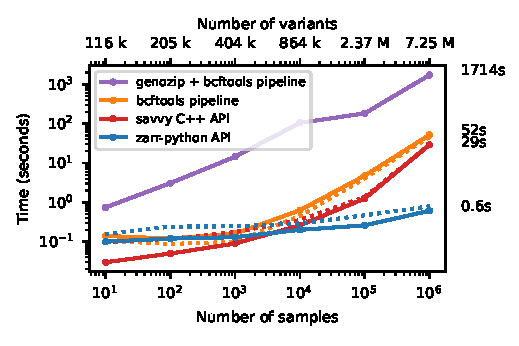
\includegraphics[width=6cm]{figures/subset-matrix-compute} &
\begin{tcolorbox}[width=7cm]
\begin{minted}[fontsize=\footnotesize]{python}
# TODO not sure how best to illustrate this. Trying out various
# options

ds = sgkit.load_dataset(ds_path)
dss = ds.isel(
    variants=slice(...),
    samples=(slice(...)))
df = sgkit_afdist(dss)

# bcftools
bcftools view PATH -S ... -r...
| bcftools +fill-tags | bcftools +af-dist

# genozip
genocat PATH -r ... -s ...
| bcftools +fill-tags | bcftools +af-dist

# Complex query
df = pd.read_csv("sample_info.csv",
    sep="\t").set_index("sample_id")
dss = ds.isel(
    samples=df.decade[ds.sample_id.values] >= 1950)
sgkit_afdist(dss)

# Corresponding shell
tail -n+2 sample_info.csv | awk '$2 >= 1950'
    | cut -f1 > samples.txt
bcftools view PATH -s samples.txt
    | bcftools +fill-tags | bcftools +af-dist

\end{minted}
\end{tcolorbox}
\end{tabular}
\caption{Whole-matrix compute performance with increasing sample size.
(A) Total CPU time required to run the afdist calculation for
a subset of 10 samples and 10000 variants from the middle of the matrix.
(B) Same for n/2 samples. Genozip did not run in this case for
$n > 10^4$ samples because it does not support a file to specify
sample IDs, and the command line was therefore too long for the shell
to execute.
(C) A simplified version of the source code used for these benchmarks.
\label{fig-subset-matrix-compute}}
\end{figure}


\subsection{Sgkit design principles}

Openness is a core organising principle of sgkit, both in terms of
development processes and code licensing, and also with respect
to usability. By following the general philosophy of array-oriented
computing, the functionality in sgkit is organised around the
key concept of a ``dataset`` which encapsulates a set of
related ``variables''. The implementation aims to be as agnostic
as possible as to the underlying implementation of these arrays,
which can be stored in-memory as NumPy arrays, in chunked
compressed on-disk storage as Zarr arrays, or ...

% Perhaps this should be mentioned in the QuantGen section?
The data layout used here is compatible with the ChromaX
breeding program simulator~\citep{younis2023chromax}, which
is leveraging other aspects of the PyData ecosystem to
fully utilise modern parallel hardware.


[In later sections we discuss enabling technologies in detail,
here we talk about how we use them from a high-level, and layout
the overall design philosophy. This isn't documentation, rather
it's the forum where we lay out explicitly early design choices
and their rationale.]

VCF conversion is handled using
\toolname{cyvcf2}~\citep{pedersen2017cyvcf2}.
[TODO any citations for these?]
BGEN using \toolname{cbgen}.
Plink support using \toolname{bed\_reader}

[Text from proposal]

The rapid evolution of supporting projects in the PyData ecosystem, including Dask for
distributed processing, Xarray for coordinated operations on groups of labeled
n-dimensional arrays, Zarr for n-dimensional array storage on cloud object
stores, and Numba for hardware acceleration. We’ve designed sgkit from the
ground up to tightly integrate with these libraries so that we can benefit from
the many improvements being made upstream, making the PyData ecosystem
accessible to statistical geneticists.

We've also defined a Zarr representation for efficient storage of this data.
We’ve designed an Xarray dataset-based data model which can be populated from
any of the file formats above, and against which library methods are
implemented. These methods include variant and sample quality control,
population structure analysis, genome-wide selection scans, and genome-wide
association analyses, including a novel implementation of the recently
developed and state-of-the-art REGENIE algorithm.



\subsection{Statistical Genetics}
Statistical genetics is largely concerned with disease associations
in humans, and the success of genome wide association studies (GWAS) has led
to explosive growth in the field~\citep{uffelmann2021genome}.
Sample size is the single most
important factor in driving statistical power, and
genotype array data has been collected for millions of samples
[more explanation and citations].
GWAS typically use genotype array data because of
its continuing cost-effectiveness, although there has been
exome~\citep{lek2016analysis,backman2021exome}
and large-scale whole genome sequence data is becoming increasingly
available~\citep{halldorsson2022sequences}.
Genotype array data is usually imputed using software such
as BEAGLE~\citep{browning2018one} or IMPUTE~\citep{howie2011genotype}.
% Mention phasing?

The \toolname{plink}~\citep{purcell2007plink} package is the most
commonly used software for GWAS and has a large range of functionality
required for quality control, association testing and analysis.
More recently software packages have emerged specifically designed
to deal with the very large sample sizes that are becoming
more prevalant, for example SAIGE~\citep{zhou2018efficiently}
Bolt-LMM~\citep{loh2015efficient}
and
REGENIE~\citep{mbatchou2021computationally} are designed to
detect associations in very large cohorts.
The Hail software [citation] has been used [to do lots of things]
[Mention qgg somewhere\citep{rohde2020qgg}]

Because of the relative homogenity of the data sources and
required tasks, programs like \toolname{plink} are able to provide
an end-to-end analysis pipline from the source genotype data, quality
control and associations via Manhattan plots.

\subsection{Population Genetics}
[Things to work in here:
1) Classically popgen is concerned with allele frequencies, and so
used a variety of different data types to access this.
2) Data was at a pretty small scale, so you could do the entire
analysis within a single monolithic package like Arlequin.
3) people have been transitioning to WGS data recently.
]

Population geneticists study evolution at the population scale,
characterising the evolutionary forces shaping the diversity
within and between populations. Compared to statistical genetics,
which is largely concerned with humans, population geneticists
study a broad range of organisms across the tree of life, both well
characterised ``model'' species, and those for which the most basic
genetic information (such as the sizes and number of chromosomes,
and ploidy level) must be determined.
Sample sizes are also much smaller,
with dozens to a few hundred genomes per species being typical.
However, projects such as Darwin Tree of
Life~\citep{darwin2022sequence} are currently sequencing tens of
thousands of different species.

% JK: I'm making this up - need to get something concrete to back it up.
% Is there any review paper summarising computation in popgen?
[THIS IS A ROUGH DRAFT: I'm just getting in a paragraph here with citations
to tools/packages that are important in PopGen. We can get a narrative
through it later.]
See \citep{excoffier2006computer} for a review of computational methods
in classical population genetics.
Because of the relatively small volumes of data and the variety
of different organisms, statistical analysis of population genetic
data has tended to be done by custom scripts. Tools such
as \toolname{plink}~\citep{purcell2007plink}
are often not applicable because of the built-in
assumptions that are appropriate only for humans and other model organisms.
Programs such as Arlequin~\citep{excoffier2005arlequin,excoffier2010arlequin}
contain a large suite of features, but can only be accessed by GUI
or command line interfaces.
BioPerl~\citep{stajich2002bioperl} and BioPython~\citep{cock2009biopython}
are more concerned with alignments and providing access to command-line
programs, and are oriented towards flexibility rather than
performance.
The \toolname{scikit-allel}~\citep{miles2023scikit}
and \toolname{pylibseq}~\citep{thornton2003libsequence}
libraries provide efficient programmatic
access to a rich suite of population genetic statistics, but have limited
support for parallelisation.

STRUCTURE~\citep{pritchard2000inference}
ADMIXTOOLS~\citep{patterson2012ancient}

% Discussion of simulated data and tree-based stuff.
Population geneticists are often interested in comparing with simulated data.
Until recently, this was done by processing
custom text formats output by programs such as
\toolname{ms}~\citep{hudson2002generating} and accompanying
scripts to compute basic statistics.
% JK: This is a bit of a self-cite fest here, but I think people would
% wonder what the connection between sgkit and tskit is if we don't
% explain it. Happy to discuss if anyone doesn't like it, though.
The \toolname{msprime}~\citep{kelleher2016efficient} simulator took a
different approach by providing a Python API which gives
access to the underlying genealogical trees, which often allow
statistics to be calculated more efficiently than standard
matrix-based approaches~\citep{ralph2020efficiently}.
These methods have been subsequently generalised to
other forms of
simulation~\citep{kelleher2018efficient,haller2018tree}
as well as being inferred from observed variation
data~\citep{kelleher2019inferring,wohns2022unified},
supported by the open-source \toolname{tskit}
library~\citep{ralph2020efficiently}.
See~\cite{baumdicker2021efficient} for further discussion on
computation in population genetic simulations, and the
\texttt{tskit} software ecosystem.
% Need to say this somewhere, or people will wonder. This is a
% rough draft
While tree-based methods are excellent for simulated data
and attractive for real-data analysis, they are not a solution
to all problems. Firstly, not all datasets are appropriate
for tree inference and secondly, before we infer trees we must
first perform extensive quality control of the raw data, necessarily
in variant-matrix form.

\subsubsection{API overview}

Sgkit provides a number of methods for computing statistics in population
genetics. All methods work on an Xarray dataset that has a number of well-known
variables defined [TODO: see section...], which for population genetics are the
genotype calls, stored in the \sgapi{call\_genotype} variable. The methods return a
new dataset containing variables that store the computed statistics.

Before running the methods, the dataset is usually divided into windows along
the genome, using the \sgapi{window\_by} functions, which tell sgkit to produce
per-window statistics. For example, \sgapi{window\_by\_position} creates windows that
are a fixed number of base pairs, while \sgapi{window\_by\_interval} creates windows
corresponding to arbitrary user-defined intervals.

It's common in population genetics to group samples into populations, which in
sgkit are referred to as \emph{cohorts}. There are two types of statistics: one-way
statistics where there is a single statistic for each cohort, and multi-way
statistics where there is a statistic between each pair, triple, etc of
cohorts. [TODO: do we need to say how cohorts are defined?]

The methods for one-way statistics include \sgapi{diversity} for computing mean
genetic diversity, \sgapi{Tajimas\_D} for computing Tajima’s D, and
\sgapi{Garud\_H} for
computing the H1, H12, H123 and H2/H1 statistics~\citep{garud2015recent}.

The methods for multi-way statistics include \sgapi{divergence} and
\sgapi{Fst} for
computing mean genetic divergence and $F_{ST}$ (respectively) between pairs of
cohorts, and \sgapi{pbs} for computing the population branching statistic between
cohort triples.

\subsubsection{Example}

We converted phased Ag1000G hypotype data in Zarr format
%[@https://www.malariagen.net/data/ag1000g-phase-2-ar1]
to sgkit's Zarr format
using the \sgapi{read\_scikit\_allel\_vcfzarr} function.
The data contained 1,164
samples at 39,604,636 sites, and was [TODO] MB on disk before conversion, and
[TODO] MB after conversion to sgkit's Zarr format. Data for the X chromosome
was discarded since it was not available for all samples. The conversion took
[TODO: X minutes Y seconds], including a postprocessing ``rechunk'' step to
ensure that the data was suitably chunked for the subsequent analysis.

We grouped samples into 15 cohorts based on location using simple Pandas and
Xarray data manipulation functions. We then set up half-overlapping windows
along the genome using sgkit's \sgapi{window\_by\_position} function with a fixed
window size of 6000 base pairs, and a step size of 3000 base pairs.

We computed H statistics for one cohort using the \sgapi{Garud\_H} function in sgkit.
This operation took [TODO: X minutes Y seconds]. Finally, we verified that the
output was concordant with scikit-allel. [TODO: how hard to reproduce the
scikit-allel visualization?]

[TODO: summarize the biologically interesting thing here]

\subsection{Quantitative Genetics}
[TODO lacking a lot of detail here in terms of compute and software.
https://github.com/pystatgen/sgkit-publication/issues/26]

Quantitative genetics is classically concerned with understanding
the link between continuously variable quantitative traits
with complex genetics~\citep{hill2010understanding}.
Through decades of selective breeding, quantitative genetics methods have
led to X-fold increases in milk yield [etc, citations].
They are also applied to
natural populations~\citep{wilson2010ecologist}
Quantitative genetics methods are used across a wide variety of
organisms, with many species of argicultural interest having
variable ploidy levels etc.

Much of classical quantitative genetics uses observed pedigree structure
in mixed models to partition the variance of phenotypes, without
reference to any genomic data.
Fitting generalised linear mixed models (LMMs) using
software such as ASReml~\citep{butler2009asreml}
and MCMCglmm~\citep{hadfield2010mcmc} require only the pedigree
information and trait data.
Genetic marker data~\citep{bernardo2008molecular} of various
types (RFLPs, microsats etc) required statistical models.
BLUPs include genetic information~\citep{endelman2011ridge}.

Many packages are available in R [cites]. Because much of the computation
in quantitative genetics has been around solving
general statistical models using linear algebra, R is very good.
However, with larger and larger samples sizes, particularly
in agricultural applications.
For example,
the 1000 bull genomes project~\citep{hayes20191000}
comprises close to 7000 genomes, embedded in multi-generation pedigrees
with millions of animals and extensive SNP array genotype and phenotype
data \citep[e.g.][]{cesarani2022mulibreed}.
[Methods are hitting a computational wall]

Much of the functionality required for quantitative genetics work
is therefore provided by access to efficient and scalable linear algebra
routines (a core element of the PyData ecosystem), the ability
to access genetic variation data from sources such as plink and VCF,
and some specialised routines to handle pedigree data and to
estimate relatedness matrices. Sgkit provides [this], with a particular
focus on supporting autopolyploids.




\subsection{Enabling technologies}

[High-level summary of where things are in terms of data analysis
in genomics, pointing forwards to
the individual use-cases of popgen, statgen etc to discuss the
individual tools.]

Other sciences have been working at the petabyte scale for some time.
[I don't really know the background here, it'll require some research.
Astronomics, geosciences etc have all been working with such large
datasets, and been using Python to do so, successfullly. Concrete
examples]

While some aspects of genomics data are unique and require specialised
tooling, by the time that variants have been called and the we wish
to work on the final stages of analysis, we are usually
working with large n-dimensional arrays of numerical data. Such
datasets are precisely what a large and active community of
developers have been working on in the PyData Ecosystem. The goal
of sgkit is to bring these tools to genomics, using a
shared platform for analysing large arrays of numerical data. In the
following subsections we discuss the key technologies, and how
they apply to genomics.

\subsubsection{Array oriented computing}

NumPy~\citep{harris2020array} has been transformational, and provides
the basic framework for scientific computing in Python.

[ Things to cite: pandas~\citep{mckinney2010data},
BioNumpy~\citep{rand2022bionumpy}, OME-Zarr~\citep{moore2023ome}]

[NOTE: we may also want a section discussing the n-dimensional array model,
but I think this section is the right place to discuss that?]

\subsubsection{Columnar binary data}

Perhaps the most important factor limiting scalability in contemporary genomics
is the continued reliance on row-wise storage of data---most often
encoded as blockwise-compressed text.
[Explain why row-wise is bad without reference to specific genomics applications.]

The Variant Call Format (VCF) is the standard method for interchanging
genomics data~\citep{danecek2011variant}.
In VCF each row describes the observations for a set of samples
at a given position along the genome, and consists of fixed columns such as the
genome position as well as per-sample columns. [More info]
VCF was introduced as part of the 1000 Genomes project, and works reasonably
well at the scale of 1000s of samples. However, when we have hundreds of
thousands of samples it becomes extremely unwieldy
. For example, the
phased genotypes for 200K samples in UK Biobank produced by Browning [cite]
require X GB of space.
(Note that this file contains no extra INFO keys; in practice a great deal
more information is stored in the VCF leading to files that are orders of
magnitude larger, and requiring them to be split into chunks, further
increasing their unwieldiness.)
Running [a simple query that requires only looking at
one column] on this file like X required Y minutes.

[TODO be more concrete here; what is the thing we're summarising?]
This slow response time to a simple query is primarily caused by the row-wise
nature of VCF (and BCF), because in order to read a single piece of
information about a particular variant site we must read \emph{all}
the information
about that site. Then, if we wish to summarise that information over
all sites, then we must read the entire dataset.

A lesser but still significant cause of inefficiency is the use of
text to store the data. [More info]

These issues are of course well known, and there are numerous projects
that seek to alleviate them. [Discuss] They're all quite bespoke to genomics data
through.

In sgkit we use Zarr which although initially introduced to store
genomics data, has now been adopted widely in [X, Y and Z].
Zarr is [description] and has [advantages]

Also to discuss (not sure how these fit in to this specific sectio
on background technologies vs existing genomics infrastructure; can
sort out later):

\begin{itemize}
\item columnar (with small records) good for I/O elimination + sequential access.
Classical locality of reference stuff as well.
\item What does this mean with ND arrays? Slippery concept. Discuss.
\item Compression improvements from columnar.
\item Poor performance of text-based VCF has been noted many times,
and lots of prior work in this space e.g. \citep{kelleher2013processing}
\item Honourable mentions for bcftools~\citep{danecek2021twelve},
htslib~\citep{bonfield2021htslib}, CRAM~\citep{bonfield2014scramble,bonfield2022cram}
which uses a columnar approach
\end{itemize}

\subsubsection{Distributed computing}

Beyond a certain scale of data there is no alternative but to
parallelise calculations across multiple computers if you wish
them to complete in a reasonable timeframe. Classically in
High Performance Computing (HPC) environments, most often used
to perform scientific computing, such distributed computing
is done using the Message Passing Interface (MPI). MPI
typically assumes a low-latency connection between nodes in
cluster, often with specialised hardware interconnects,
and can be used very effectively to [do things like solve big PDEs].
However, MPI is [hard to program and hard to run], and applications
in genomics have been limited to [things like the ABySS assembler].

[Paragraph describing, Big data, Hadoop, MapReduce, Spark, etc. Why
they don't use MPI, that the problem being solved was/is.
Applications to genomics like ADAM~\citep{nothaft2015rethinking} were promising, but never really
took off. Hail (see also genomics section) notably does a
bunch of things well, but only by rewriting whole chunks of the
underlying technologies]

We use Dask [for reasons].

\subsubsection{Just-in-time compilation}

Many of the analyses that we wish to perform in genomics are unique,
and the ability to quickly put together complex queries using
high-level tools like shell pipelines and scripting languages
is often a major bonus. However, such approaches are often not
viable at the petabyte scale, where efficient compiled code that
uses available CPU resources effectively are required. However,
writing code in compiled languages such as C, C++ or Java
is far more labour intensive, as well as requiring more specialised
software development experience.

Similarly, [scripting languages such as python are great for
contributing to open source libraries, because there's a much
lower barrier to contribution.]

We use numba because [it's awesome].

\subsubsection{Heterogenous computing}

GPUs are cool, we support them.


\subsection{Storing genetic variation data}
The shortcomings of VCF (and to a lesser degree, BCF) as a storage
format and the basis of efficient computation have long been
recognised \citep[e.g.][]{kelleher2013processing,layer2016efficient,li2016bgt},
and many alternatives
have been proposed.

Purely archival formats try to get the maximum possible compression levels,
without much attention to query performance. Typically these use
highly specialised approaches to maximise compression performance
on genotype data.

These include:
TGC~\citep{deorowicz2013genome}
GTShark~\citep{deorowicz2019gtshark},
VCFShark~\citep{deorowicz2021vcfshark}.

SpVCF~\citep{lin2020sparse} is an extension of the VCF text
format that maximises compatibility, while gaining substantial
improvements in file sizes.

Many tools focus on balancing compression performance with
being able to run queries, typically outputting a VCF.
e.g.
BGT~\citep{li2016bgt},
GQT~\citep{layer2016efficient},
SAVVY~\citep{lefaive2021sparse},
XSI~\citep{wertenbroek2022xsi},
GTC~\citep{danek2018gtc},
GTRAC~\citep{tatwawadi2016gtrac}
genozip~\citep{lan2020genozip,lan2021genozip}
GBC~\citep{zhang2023gbc}.

SeqArray~\citep{zheng2017seqarray} and the GDS format~\citep{zheng2012high}
provide efficient storage and programmatic access in R.


Many recent tools are based on the Positional Burrows--Wheeler
Transform (PBWT)~\citep{durbin2014efficient}, which takes advantage
of the underlying haplotype structure of genomic data to provide
concise storage, and efficient haplotype matching.

The approach taken by \toolname{plink}~\citep{purcell2007plink,chang2015second} is to
store data in an uncompressed binary format. This has some major
advantages.

BGEN \citep{band2018bgen} is optimised for storing large-scale
genotype array data and stores probabilities, and is used
in particular by UK Biobank~\citep{bycroft2018genome}
[Should consider the "hard-call" nature of most of these formats]

Many methods working with large scale genetic
data now use the PBWT or variants of
it~\citep[e.g.][]{li2016bgt,lefaive2021sparse,wertenbroek2022xsi}. PBWTs have
disadvantages, however: data must be phased, and compression level
is quite sensitive to the presence of errors [citation? people have
worked around this]

Several tools provide querying interfaces in their CLIs
(reminiscent of SQL) to provide easy access to particular samples, or
variants~\cite{li2016bgt,layer2016efficient}.

More recently XSI~\citep{wertenbroek2022xsi} is an file format that
uses a combination of strategies to achieve excellent compression
performance, and can support some calculations directly on the
compressed format. It provides a command line interface and a
C API.

The SAV format is an extension of BCF that takes advantage
of the sparseness of large scale genomic datasets~\citep{lefaive2021sparse}.
They provide a command line interface and a C++ API.

It is important to note that the example in Fig.~\ref{fig-data-storage}
is something of a best-base
scenario in terms genomic dataset storage, in that we are only
storing genotype data (per sample, per variant),
and, because it is error-free, is very
highly compressible. Noisier genotypes will not compress quite
so well, and storing less compressible data (such as genotype
quality values) results in a large increase in the overall
storage size. This is essentially unavoidable, but the Zarr-based
approach still has some significant advantages over VCF/BCF
[basically we can store separately and come up with distinct
compression strategies based on the data type. Dunno if we
want to get into this here. This is a complex topic with
a lot of existing work which we should review and reference,
and this is maybe not the place to do it.].

[SpVCF has some good text on high-entropy QC measures. We have to
reduce this entropy or we just can't store the data]


[Why are we reviewing all this? Well, we want to make the point
that people have been trying hard to address the problem of
how to deal with large-scale genomic data for quite a while,
and have come up with lots of specialised methods. There
are a few things to keep in mind. Our approach is to use
standard methods just on the "rectangles" of variant data
and it's already quite good. You could imagine writing specialised
compression filters for genotypes, if you wanted (maybe a
discussion item though). The key thing is the \emph{interface}.
They're all tying to the command line and to classical
sequential workflows. We have Python, and distributed compute. ]

% TEXT from HSG chapter section on compressing data

% The simplest approach to compressing such data is to organise it in a
% `variant-centric' fashion, such that all observed genotypes for a given variant
% are stored in a contiguous block. Because most variants are rare, this will
% result in long runs of identical values that compress well using standard
% methods. This is the approach taken by the Variant Call
% Format~\citep{danecek2011variant}, and its more efficient binary encoding, BCF.
% The compression levels achieved by this straightforward approach are good, and
% quite competitive with more sophisticated methods. The disadvantage
% is that many queries require full decompression of the data, which can be
% prohibitively time-consuming. The SpeedGene data format and software
% library~\citep{qiao2012handling} chooses from one of three encoding methods for
% each SNP determined by the allele frequency; \cite{sambo2014compression} extend
% this idea by identifying blocks of SNPs in LD, and adding two additional
% potential encodings utilising this information.

% An alternative to this variant-centric approach is to store genotypes in a
% `sample-centric' fashion. Here, all genotypes for a particular sample are
% stored consecutively. While this breaks the simple repetition structure of data
% stored in variant-centric form, other methods can be employed to find
% compressible structure. For example, TGC~\citep{deorowicz2013genome} compresses
% sample genotypes using a custom Lempel-Ziv style approach on runs of identity
% among samples. This explicit use of LD structure results in excellent
% compression performance (for example, 32MB for all SNPs in 1000 Genomes
% chromosome 1); unfortunately, querying a dataset requires full decompression,
% making the format unsuitable for online analysis. The GQT
% toolkit~\citep{layer2016efficient} also uses the sample-centric organisation of
% genotype data, but takes a different approach to compression. Variants are
% sorted by allele frequency (resulting in longer runs of identical values within
% samples) and then compressed using an efficient bit-vector
% representation~\citep{wu2002compressing}. The resulting file-sizes are similar to
% compressed BCF, but many queries can be performed directly on the compressed
% representation and are therefore many times faster.

% The positional Burrows-Wheeler transform~\citep{durbin2014efficient}, or PBWT,
% is another sample-centric method. Building on the success of Burrows-Wheeler
% transform applications in
% genomics~\citep{langmead2009ultrafast,li2009fast,li2009soap2}, PBWT provides
% very good compression performance and efficient algorithms for finding
% haplotype matches. The algorithm builds a representation of the data based
% on sorted haplotype prefixes in linear time, and the LD structure of the data
% ensures that the sorting orders between adjacent sites change very little
% on average. The method has been successfully applied
% to phasing~\citep{loh2016reference}, detection of IBD
% segments~\citep{naseri2017ultra}, improving the performance of the Li and
% Stephens model~\citep{lunter2016fast}, and a general query engine for genotype
% data~\citep{li2016bgt}. Recent extensions include privacy preserving
% search~\citep{shimizu2016efficient} and generalisation to the setting of graph
% genomes~\citep{novak2017graph}.

\subsection{Reimplementing complex methods}


To showcase the advantages of \sgkit's pure-Python development model, we
discuss some things we've implemented.


\subsection{Functionality}

[Just listing out all the things that have been implemented to try and get
some kind of grip on what we're doing]


\begin{itemize}

\item \sgapi{pc\_relate} estimate genetic relatedness, returns sample x sample
kinship coefficient matrix. \citep{conomos2016model} (genetic Relatedness matrix)

\item \sgapi{Weir\_Goudet\_beta} sample x sample Kinship matrix
\citep{weir2017unified} (genetic Relatedness matrix)

\item \sgapi{genomic\_relationship} Genetic relationship matrix estimated
by either the Van Raden algorithm generalised to
autopolyploids~\citep{vanraden2008efficient,ashraf2016estimating,bilton2020developing}
and the Endelman-Jannink estimator \citep{endelman2011ridge}
(genetic Relatedness matrix)

\item \sgapi{hybrid\_relationship} Hybrid relationship matrix
(AKA the HRM or H-matrix) combining pedigree and genomic information
~\citep{martini2018effect}
Also \sgapi{hybrid\_inverse\_relationship} (Relatedness matrices)

\item \sgapi{pedigree\_inverse\_kinship} Calculate the inverse of the kinship
matrix from pedigree structure.

\item \sgapi{pedigree\_kinship} Calculate the kinship
matrix from pedigree structure.

\item \sgapi{invert\_relationship\_matrix} Compute the inverse of a
relationship matrix (?)

\item \sgapi{pedigree\_contribution} expected genomic contribution of each
sample to each other based on pedigree (Hamilton-Kerr?)

\item \sgapi{pedigree\_inbreeding} Estimate expected per-sample
inbreeding coefficients from pedigree structure.
\citep{hamilton2018computation}

\item \sgapi{identity\_by\_state} Pairwise sample x sample matrix
of IBS probabilities

\item \sgapi{ld\_matrix} Sparse matrix of LD values exceeding a threshold.
\item \sgapi{ld\_prune} Find a maximally independent set of variants
(based on plink algorithm)

\item \sgapi{regenie} produces trait estimates for association tests.
\citep{mbatchou2021computationally} (GWAS)
\item \sgapi{genee} Gene-level effects
\citep{cheng2020estimation} (GWAS)
\item \sgapi{gwas\_linear\_regression} Least square regression based
on BoltLMM~\citep{loh2015efficient} (GWAS)
\item \sgapi{hardy\_weinberg\_test} Exact Hardy-Weinberg
test~\citep{wigginton2005note} (GWAS)

\item \sgapi{TajimasD} popgen stat
\item \sgapi{divergence} popgen stat
\item \sgapi{diversity} popgen stat
\item \sgapi{pbs} popgen stat
\item \sgapi{Fst} popgen stat
\item \sgapi{Garud\_H} soft sweep stats~\citep{garud2015recent}


\item \sgapi{sample\_stats} basic QC variant data

\item \sgapi{variant\_stats} basic QC variant data

\item \sgapi{pedigree\_sel} slice by pedigree

\item \sgapi{window\_by\_genome} Windowing

\end{itemize}





\section{Discussion}

Outline of a possible narrative by paragraph:
\begin{itemize}
\item When VCF was introduced as part of the work of the 1000 Genomes
project the software landscape was a real mess. It has entirely
succeeded in standardising the output of variant callers, and methods
have interoperated well for the past decade. As a method of interchange
following classical file-oriented paradigms it works well enough.
It is also a good archival format: when compressed with a well established
method like gzip and combined with the well-documented description of
the text, we can be sure that files will still be readable decades
from now.

\item VCF is holding back large-scale genomics, however, and in particular the
analysis of population scale genetic variation datasets like UKB and GeL.
Describe the current state of affairs. Variant datasets are chunked up
into reasonable sized bits (10s of gigabytes) so that they can be processed
in parallel. Doing anything with them requires interacting with workflow
managers. In practise, it is not possible to directly write programs to
work across multiple large-scale datasets: although the chunks of data
are given in VCF, orchestrating how the chunks are processed and
the results combined involves substantial work, involving the workflow
manager, and the details of how chromosomes are split into chunks.
Cite examples like the phasing pipelines for UKB from Brownings etc.

\item Distributed computing is the reality, and increasingly datasets
are being mandatorily stored in public clouds as part of
Trusted Research Environments. Cloud object stores are the reality
because it is much cheaper. POSIX file systems are emulated on top of
this. Benefits of breaking up data into manageable pieces are that
compute resources can be localised to the data. Compute resources are
most effectively obtained as short-lived, small VMs that operate
as part of a large cluster. Large vertically scaled ``pet'' servers
are much more expensive, and just not feasible for the current
scale of data. Lots of other architectural
benefits from the new reality of cloud-based storage.

\item Classical methods based around Unix pipelines and streaming
files between processes on a single machine are therefore a
significant mismatch to the reality of large-scale genetic variation
datasets. The majority of methods suggested to make working
with VCF data more efficient are based on these ideas: they all
create a single large file and regard distribution of work
in a cluster as extrinsic. Most output VCF as the result of queries,
which also assumes that the VCF data can be efficiently processed.
This is a reasonable assumption for thousands of samples, but not
for larger datasets.

\item The key issue here is that VCF is not a \emph{computational}
format. Contrast VCF with plink, which stores data on disk in a
form that can be computed on directly. Plink is limited in what
can be descibed though, does not compress, and is not designed
to distributed.

\item The large-scale analysis of genetic variation data does not
need a more efficient file format, which allows files to be downloaded
somewhat more quickly, and subsets extracted somewhat more efficiently
as VCF. It needs a standard storage platform that allows data to be
processed directly without conversion, subsetted efficiently across
both the variant and sample dimensions, with first-class support
for all the necessary additional information (GT values etc),
and that is suited to the realities of today's cloud-based
storage and processing facilities.

\item We suggest that the model used by Zarr is a good choice for this.
We have shown that chunks of the genotype matrix compressed with standard
methods are competitive with highly specialised methods for
genotype data. In reality most of the storage is for non-genotype
data anyway, where everyone is essentially doing the same thing.
Columnar storage allows getting just (e.g.) the variant positions
without reading everything. Another benefit is that by storing
fields separately in different cloud objects, they can have
different permissions. So, users can be given differential access
to read parts of the dataset, and this is managed directly
by the cloud storage. Give example.

\item A major strong point of Zarr is its simplicity. All it's doing
is compressing n-dimensional chunks of numerical data and storing
them using fixed address keys. This key-value approach means that storage
is very flexible and implementation is straightforward. There
are several implementations of the Zarr protocol, and while some of these
are rudimentary, they could be improved or replaced with relatively
little effort. Zarr has been successfully used to store petabytes
of data across different sciences --- genetic variation data is largely
arrays of numerical data, and not really that different ultimately.
Zarr is cloud native.
Zarr is an open specification, built on standard components (contrast
with Hail).

\item Zarr is not perfect. Discuss limitations around ragged arrays,
etc. Forthcoming improvements in zarr v3. The whole genotype matrix
paradigm is challenged by graph genomes as well. While this is
being worked out, there is still plenty of data to analyse as a
genotype matrix.

\item Vision. An ecosystem of tools that interoperate
based on an open, cloud-based format where distribution is naturally
managed by the stored chunks. Tools can be run on different datasets
with minimal tuning, not by writing a full layer of orchestration.
Tools read the data they need, not the entire dataset. Users read
directly from a single canonical dataset, and do not maintain
their own filtered copies. We suggest that the Zarr VCF approach
we have provided would be a good starting point for designing
such a compute platform.

\item TODO several missing paragraphs here discussing the
benefits of the other layers of the stack.

\item Closing. Sgkit, built on the fundamental idea of storing
data in a simple, efficient and distributable fashion, would
hopefully be one element of this compute ecosystem.
Xarray, Dask and numba provide powerful tools to make users
more productive, and enable the interactive analysis of large
scale variation data. We have illustated the current functionality
through examples here across X-genetics, but there is much
potential for more. The library is specifically designed to make
contribution easy, and we welcome people to the open-source
community.

\end{itemize}


%%% OLD TEXT
% \begin{itemize}

% \item While API based approaches such as htsget~\citep{kelleher2019htsget}
% and more generally federated access to data~\citep{rehm2021ga4gh}
% are an important part of the future of genomics, we must still pay
% attention to how efficient \emph{local} compute is. We need to
% store and exchange data in an efficient and easily accessible
% format. [Could talk about
% how early GA4GH APIs failed because they didn't really consider
% efficiency? Converting VCF to JSON was never going to be efficient?
% Might not be worth getting into]

% \item Users of sgkit will be able to perform data manipulation, analysis, and
% visualization using familiar PyData tools, with only domain-specific methods
% requiring domain-specific APIs. They will also benefit from interactive
% performance for medium-sized data and the ability to scale out to biobank-scale
% data within the same library. 

% \item
% Methods developers won’t have to reimplement undifferentiated functionality
% like defining a custom data model, reading from files into that data model, and
% validating data. Instead, they can implement their novel methods against
% sgkit’s data model and instantly gain adjacent functionality and accessibility
% to sgkit’s user community. This is well illustrated by our implementation of
% the state-of-the-art REGENIE algorithm, which requires less than 1000 lines of
% Python code (including documentation) and has comparable performance to the
% original C++. Further, many key methods in statistical genetics operate on GWAS
% summary statistics, and integrating individual level data with external summary
% statistics is an increasingly important strategy which other toolkits have not
% yet formalized.

% \item sgkit makes it easier for researchers to
% make their whole analysis pipeline available in a reproducible Jupyter
% notebook. Most statistical genetics papers describe the collection of
% command-line utilities used in their methods section, and a select few make a
% workflow connecting the command-line utilities available. Users of sgkit can
% work within a Jupyter notebook without having to call out to command-line
% utilities, making the journey from raw data to scientific findings easier to
% represent in a single notebook.

% \end{itemize}

\section{Methods}

\subsection{Benchmarking}
Full details of the benchmarking done in
Figure~\ref{fig-data-storage} and
Figure~\ref{fig-whole-matrix-compute}.
Quick notes:

\begin{itemize}
\item Dataset is based on subsets of French-Canadian sims. We simplify
for increasingly large subsets, keeping only variant sites. We then
convert to VCF and encode to BCF using
\texttt{tskit vcf | bcftools view -O b}.
\item We used a chunk size of XX for sgkit, after some experimentation.
This gave n files of around x MB each for the ``call\_genotypes`` array.
We used the defaults for savvy and genozip.
\item For the afdist CPU time we measure the sum of the total user and
system times required to execute the full command, as reported by GNU
time. Each tool was instructed to use one thread, where the options
were provided. For genozip, the time required to compute
\texttt{genocat file.genozip | bcftools +af-dist}. Because commands
in the pipeline execute concurrently on mutiple cores, the total CPU time is
greater than the elapsed time.
\item For the threading speedup plot, we report the time required to compute
afdist with 8 threads relative to 1 thread (a speedup of 8 is therefore
the maximum). For savvy, our C++ implementation of afdist calculates
on 8 chunks of genome, and aggegates once they are completed.
Bcftools has a ``--threads`` option, but it only applies to decoding.
\item Where possible in pipelines we use uncompressed BCF
 output \texttt{-Ou} to make processing more efficient (skip printf
and parsing costs, which are substantial).
\item We do not use BCF output in genozip because it doesn't support
it directly, only VCF (supports BCF by pipeing through bcftools).
\end{itemize}
\section{Acknowledgments}

\bibliography{paper.bib}

% \subsection{Level 2 Heading}

% \subsubsection{Level 3 Heading}

% \paragraph{Level 4 Heading}

%%%%%%%%%%%%%%%%%%%%%%%%%%%%%%%%
% Example Table:
%%%%%%%%%%%%%%%%%%%%%%%%%%%%%%%%
% \begin{table}[bt]
% \caption{\label{tab:example}Automobile Land Speed Records (GR 5-10).}
% % Use "S" column identifier to align on decimal point
% \begin{tabular}{S l l l r}
% \toprule
% {Speed (mph)} & Driver          & Car                        & Engine    & Date     \\
% \midrule
% 407.447     & Craig Breedlove & Spirit of America          & GE J47    & 8/5/63   \\
% 413.199     & Tom Green       & Wingfoot Express           & WE J46    & 10/2/64  \\
% 434.22      & Art Arfons      & Green Monster              & GE J79    & 10/5/64  \\
% 468.719     & Craig Breedlove & Spirit of America          & GE J79    & 10/13/64 \\
% 526.277     & Craig Breedlove & Spirit of America          & GE J79    & 10/15/65 \\
% 536.712     & Art Arfons      & Green Monster              & GE J79    & 10/27/65 \\
% 555.127     & Craig Breedlove & Spirit of America, Sonic 1 & GE J79    & 11/2/65  \\
% 576.553     & Art Arfons      & Green Monster              & GE J79    & 11/7/65  \\
% 600.601     & Craig Breedlove & Spirit of America, Sonic 1 & GE J79    & 11/15/65 \\
% 622.407     & Gary Gabelich   & Blue Flame                 & Rocket    & 10/23/70 \\
% 633.468     & Richard Noble   & Thrust 2                   & RR RG 146 & 10/4/83  \\
% 763.035     & Andy Green      & Thrust SSC                 & RR Spey   & 10/15/97\\
% \bottomrule
% \end{tabular}

% \medskip
% Source: \url{https://www.sedl.org/afterschool/toolkits/science/pdf/ast_sci_data_tables_sample.pdf}

% \tabledata{This is a description of a data source.}\label{tabdata:first}
% \tablesrccode{This is a description of a source code.}\label{tabsrccode:first}

% \end{table}

%%%%%%%%%%%%%%%%%%%%%%%%%%%%%%%%%%%%%%%%%%%%%%%%%%%%%%%%%%%%
% feature box
%%%%%%%%%%%%%%%%%%%%%%%%%%%%%%%%%%%%%%%%%%%%%%%%%%%%%%%%%%%%

% \begin{featurebox}
% \caption{This is an example feature box}
% \label{box:simple}
% This is a feature box. It floats!
% \medskip

% \includegraphics[width=5cm]{example-image}
% \featurefig{`Figure' and `table' captions in feature boxes should be entered with \texttt{\textbackslash featurefig} and \texttt{\textbackslash featuretable}. They're not really floats.}

% \lipsum[1]
% \end{featurebox}

%%%%%%%%%%%%%%%%%%%%%%%%%%%%%%%%%%%%%%%%%%%%%%%%%%%%%%%%%%%%
% Figures
%%%%%%%%%%%%%%%%%%%%%%%%%%%%%%%%%%%%%%%%%%%%%%%%%%%%%%%%%%%%

% \begin{figure}
% \includegraphics[width=\linewidth]{elife-13214-fig7}
% \caption{A text-width example.}
% \label{fig:view}
% %% If the optional argument in the square brackets is "none", then the caption *will not appear in the main figure at all* and only the full caption will appear under the supplementary figure at the end of the manuscript.
% %
% \figsupp[Shorter caption for main text.]
% {This is a supplementary figure's full caption, which will be used at the end of the manuscript.
%   \figsuppdata{A data source; see \url{https://doi.org/xxx}}
%   \figsuppdata{Another data source.}
%   \figsuppsrccode{And the source code.}}
% {\includegraphics[width=6cm]{frog}}\label{figsupp:sf1}
% %
% %
% \figsupp{This is another supplementary figure.}
% {\includegraphics[width=6cm]{frog}}
% %
% %
% \videosupp{This is a description of a video supplement.}\label{videosupp:sv1}
% \figdata{This is a description of a data source.}\label{figdata:first}
% \figdata{This is another description of a data source.}\label{figdata:second}
% \figsrccode{This is a description of a source code.}\label{figsrccode:first}
% \end{figure}


%%%%%%%%%%%%%%%%%%%%%%%%%%%%%%%%%%%%%%%%%%%%%%%%%%%%%%%%%%%%
%%% APPENDICES
%%%%%%%%%%%%%%%%%%%%%%%%%%%%%%%%%%%%%%%%%%%%%%%%%%%%%%%%%%%%

% \appendix
% \begin{appendixbox}
% \label{first:app}
% \section{Firstly}
% \lipsum[1]

%% Sadly, we can't use floats in the appendix boxes. So they don't "float", but use \captionof{figure}{...} and \captionof{table}{...} to get them properly caption.
% \begin{center}
% \includegraphics[width=\linewidth,height=7cm]{frog}
% \captionof{figure}{This is a figure in the appendix}
% \end{center}

% \section{Secondly}

% \lipsum[5-8]

% \begin{center}
% \includegraphics[width=\linewidth,height=7cm]{frog}
% \captionof{figure}{This is a figure in the appendix}
% \end{center}

% \end{appendixbox}

% \begin{appendixbox}
% \includegraphics[width=\linewidth,height=7cm]{frog}
% \captionof{figure}{This is a figure in the appendix}
% \end{appendixbox}

\clearpage
\renewcommand\thefigure{S\arabic{figure}}
\setcounter{figure}{0}
\renewcommand\thetable{S\arabic{table}}
\setcounter{table}{0}

\section*{Supplementary Material}

\begin{figure}[ht]
	\begin{center}
		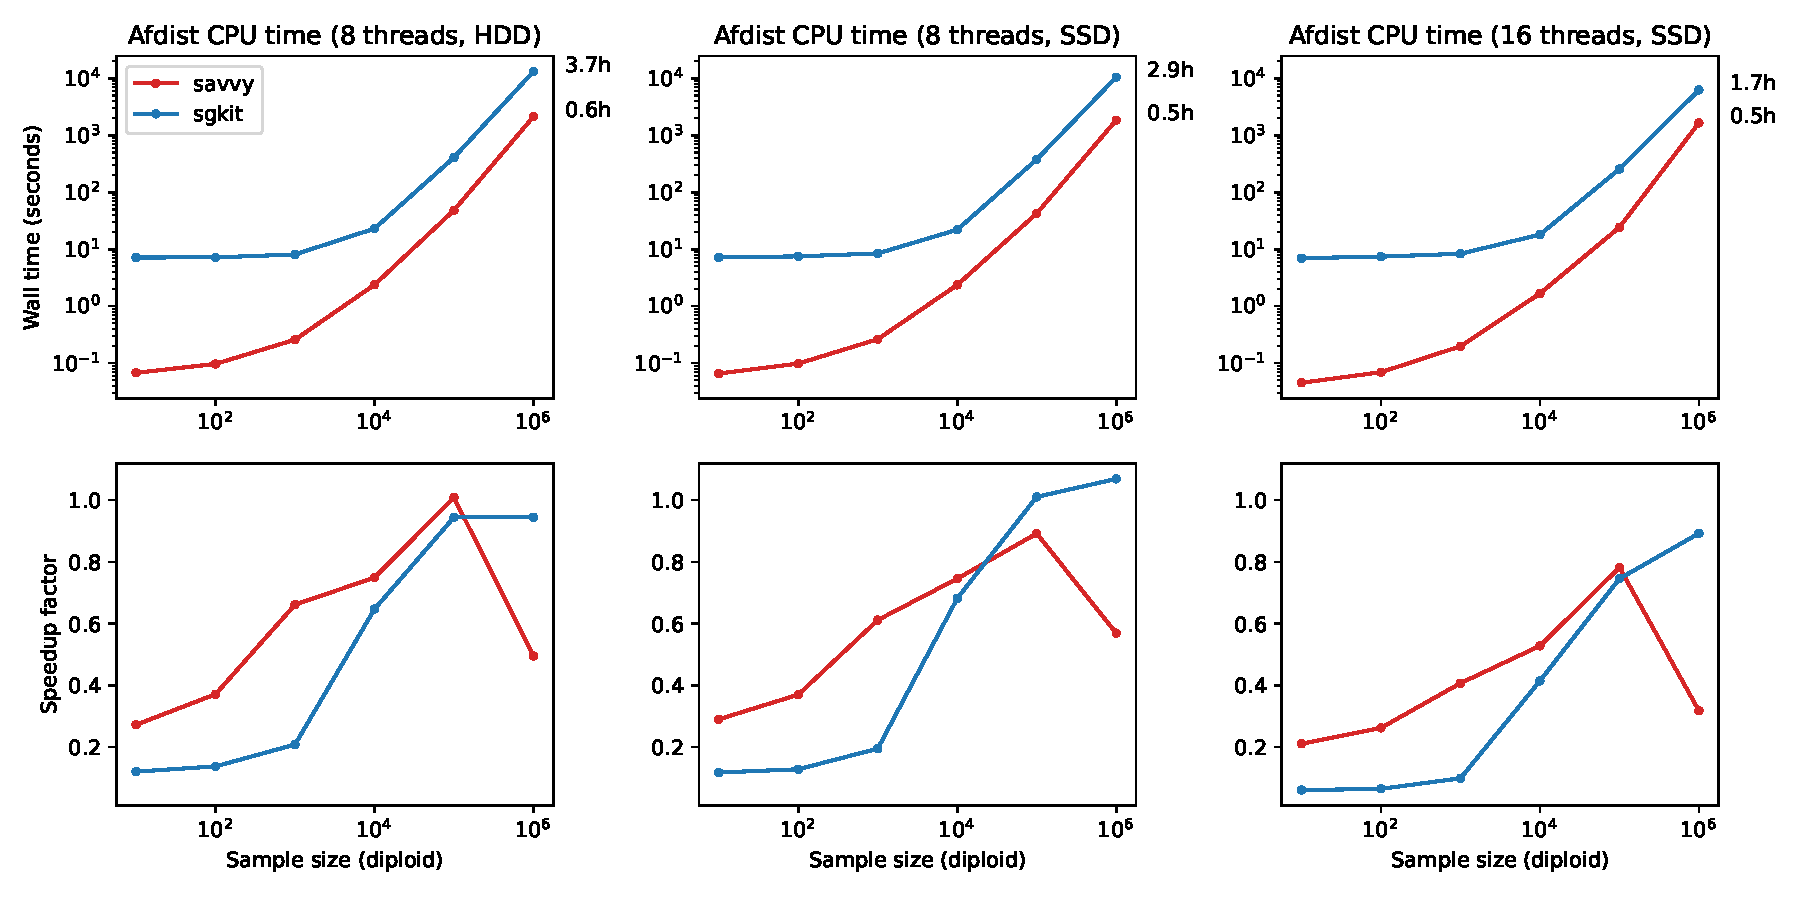
\includegraphics[width=\textwidth]{figures/whole-matrix-compute-supplemental}
	\end{center}
	\caption{\label{fig-whole-matrix-compute-supplemental}
    Limitations of vertical scaling on whole-matrix afdist. The elapsed
wall-clock time required to compute afdist on the whole genotype matrix using
different numbers of threads and storage backends (top row), and the relative
speedup obtained from threads as a fraction of optimum speedup (bottom row).
[TODO more detail and link to fig 1. Also add the times for bcftools and
genozip in col 1?]
}
\end{figure}

\end{document}
